\apendice{Documentación técnica de programación}

\section{Introducción}
El propósito de esta sección es la documentación de los componentes internos del proyecto y los aspectos más relevante de su desarrollo a nivel técnico, orientado a aquellas personas con conocimientos en informática interesadas en el desarrollo del mismo.

\section{Estructura de directorios}
El repositorio del proyecto, \textbf{accesible en la siguiente URL:} \url{https://github.com/AlbertoPorres/autograder-python}, cuenta con la siguiente estructura de directorios:
\begin{itemize}
\tightlist
\item \textbf{/:} Directorio raiz del proyecto. Contiene el fichero README y LICENSE para el proyecto, el archivo \textit{app.py} de ejecución de la aplicación, el archivo de requirements y Dockerfile para su instalación dentro de un contenedor Docker, el archivo de configuración de Jupyter Notebook y el resto de directorios del proyecto.
\item \textbf{/env:} Carpeta correspondiente a VirtualEnv donde se encuentran instaladas todas las dependencias de la aplicación para su correcta ejecución en el ambiente de desarrollo.
\item \textbf{/migrations:} Directorio de migraciones de la Base de Datos realizadas durante el desarrollo del proyecto.
\item \textbf{/src:} Directorio de código fuente del proyecto. En él se encuentra el archivo \textit{\_\_init\_\_.py} de configuración del proyecto flask, el archivo \textit{forms.py} correspondiente al manejo de formularios mediante Flask-Forms, el archivo \textit{management.py} correspondiente al manejo de la API de Nbgrader, el archivo \textit{models.py} correspondiente a los modelos de datos de SQLAlchemy, el archivo \textit{routes.py} donde se realizan las labores de controlador y la base de datos \textit{database.db} de la aplicación.
\item \textbf{/src/courses:} se encuentra el curso base que es utilizado como plantilla para la creación de nuevos cursos. En este directorio se almacenarán todos los cursos que se creen en la aplicación mediante el copiado y renombrado del curso base.
\item \textbf{/src/courses/base\_course:} curso base que contiene todos los directorios necesarios para el funcionamiento de Nbgrader (autograded, content, feedback, release, source y submitted), un notebook vacío utilizado para la creación de nuevas tareas dentro del curso mediante el copiado y renombrado del mismo, el archivo de configuración de Nbgrader \textit{nbgrader\_config.py}, la base de datos de Nbgrader \textit{gradebook.db} y un directorio adicional \textit{content} en el que se almacenan los archivos de contenido teórico de las secciones del curso.
\item \textbf{/src/static:} Contenidos estáticos de la aplicación. En él se encuentra el directorio de imégenes y el archivo \textit{base.css} de estilos.
\item \textbf{/src/static/imagenes:} Directorio de imágenes.
\item \textbf{/src/templates:} Directorio de archivos HTML.
\item \textbf{/doc:} Directorio documentación del proyecto.
\item \textbf{/doc/tex:} Directorio de archivos .text de la documentación.
\item \textbf{/doc/img:} Directorio de imágenes de la documentación.
\item \textbf{/Curso-Python:} Este directorio contiene los contenidos teóricos y tareas del curso de introducción a Python el cual ha sido añadido a la plataforma tras su despliegue vacío. Este contiene las 6 secciones de contenidos correspondientes a este curso (Introducción, Funciones, Listas y Tuplas, Control de Flujo, Diccionarios y Orientación a Objetos) divididas cada una en un directorio particular con su respectivo nombre. Dentro de cada directorio-sección se encuentran dos notebooks (archivos ipynb), el primero correspondiente al archivo de contenido teórico de la sección y cuyo nombre empieza por ''T\_'' (teoría) y el segundo correspondiente al archivo tarea en versión del profesor y cuyo nombre empieza por ''EV\_'' (evaluación).  

\end{itemize}

\section{Manual del programador}
Este manual tiene como objetivo dar información a futuros programadores que trabajen en el proyecto sobre los aspectos más importantes del código y herramientas de este.

\subsection{Prueba Nbgrader}
Tras considerar diversas herramientas de autocorrección de ejercicios \textit{Nbgrader} fue seleccionada como la herramienta de autograding a utilizar en nuestro proyecto. En esta sección queda documentada la primera toma de contacto con la herramienta en la que se realizó la instalación y prueba de esta. A diferencia de nuestro proyecto, en el cual las acciones de generación y corrección automática de tareas se realizan mediante el uso de la API pública de Nbgrader, en este primer manejo de la herramienta se hizo uso de la intefaz de usuario adicional que esta proporciona denominada Formgrader. Pese a ello, esta prueba demuestra la estructura de directorios de la que Nbgrader depende y nos proporciona nociones importantes sobre su funcionamiento:

\subsubsection{Instalación y preparación de ficheros}

Puesto que Nbgrader es un software de autocorreción de pruebas dependiente de Jupyter Notebook, el proceso de preparación de la herramienta para esta prueba fue el siguiente:

\begin{enumerate}
\item Instalación de la herramienta desde el terminal de Jupyter:

\begin{figure}[H]
    \centering
    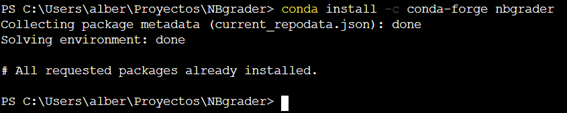
\includegraphics[width=0.8\textwidth]{img/instal/instal_1.png}
    \caption{Proceso de instalación 1}
\end{figure}

\item Debido a la forma en la que nbgrader busca las tareas y test y opera con ellos, se debe de crear una estructura concreta de ficheros en el directorio raíz. En primer lugar, se crea el fichero “submitted” (enviados) en el que se almacenarán las tareas enviadas por los alumnos:

\begin{figure}[H]
    \centering
    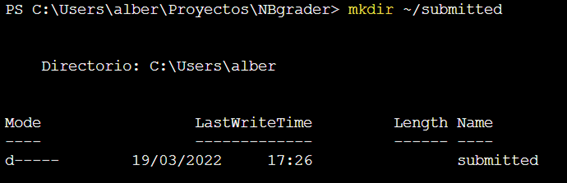
\includegraphics[width=0.8\textwidth]{img/instal/instal_2.png}
    \caption{Proceso de instalación 2}
\end{figure}

\item Dentro del directorio “submitted” se debe de incluir un fichero para las entregas de cada alumno, en este caso solo tendremos al alumno “alum1”:

\begin{figure}[H]
    \centering
    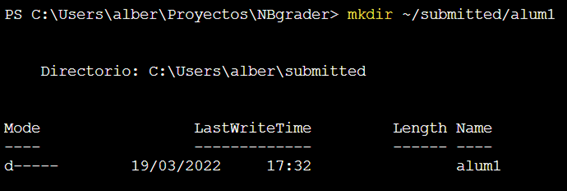
\includegraphics[width=0.8\textwidth]{img/instal/instal_3.png}
    \caption{Proceso de instalación 3}
\end{figure}

\item Dentro de los ficheros individuales de cada alumno se debe crear un fichero por cada tarea encargada, en este caso definimos una única tarea, “task1”:

\begin{figure}[H]
    \centering
    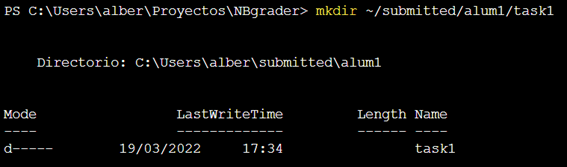
\includegraphics[width=0.8\textwidth]{img/instal/instal_4.png}
    \caption{Proceso de instalación 4}
\end{figure}

\item Los ficheros tareas enviadas por los alumno almacenadas en estas carpetas tendrán el mismo nombre que la carpeta de esa tarea correspondiente con una extensión .ipynb (notebook de jupyter).

\end{enumerate}


\subsubsection{Lanzamiento y creación de una tarea}

\begin{enumerate}
\item Una vez creada la estructura de ficheros reiniciamos jupyter notebook:	

\begin{figure}[H]
    \centering
    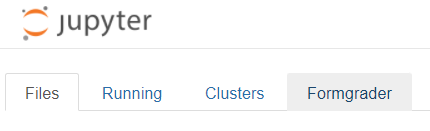
\includegraphics[width=0.8\textwidth]{img/prueba/prueba_1.png}
    \caption{Proceso de lanzamiento y creación 1}
\end{figure}

\item Al reiniciarlo nos habrá aparecido una nueva sección (Formgrader). En esta sección podremos gestionar la creación de tareas para los alumnos a través de la UI Formagrader:

\begin{figure}[H]
    \centering
    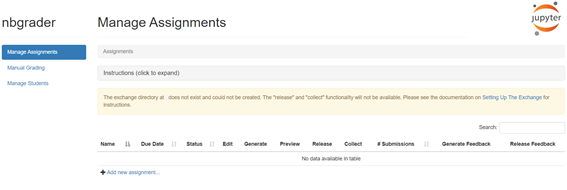
\includegraphics[width=0.8\textwidth]{img/prueba/prueba_2.png}
    \caption{Proceso de lanzamiento y creación 2}
\end{figure}

\item Para crear una nueva tarea, hacemos click en la opción “Add new assigment” y rellenamos los campos:

\begin{figure}[H]
    \centering
    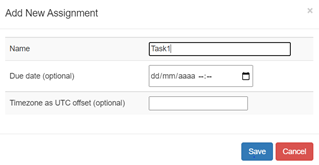
\includegraphics[width=0.8\textwidth]{img/prueba/prueba_3.png}
    \caption{Proceso de lanzamiento y creación 3}
\end{figure}

\begin{figure}[H]
    \centering
    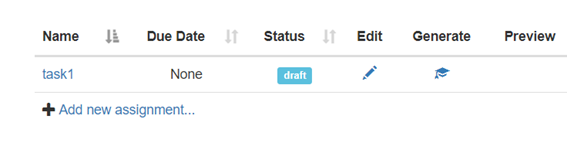
\includegraphics[width=0.8\textwidth]{img/prueba/prueba_4.png}
    \caption{Proceso de lanzamiento y creación 4}
\end{figure}

\item Para editar la tarea hacemos click en el nombre:

\begin{figure}[H]
    \centering
    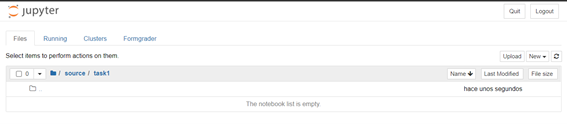
\includegraphics[width=1\textwidth]{img/prueba/prueba_5.png}
    \caption{Proceso de lanzamiento y creación 5}
\end{figure}

\item En esta sección creamos una nueva tarea (notebook) y editamos su nombre. Dentro del apartado de “view” (vista) podemos activar el modo de creación de tareas:

\begin{figure}[H]
    \centering
    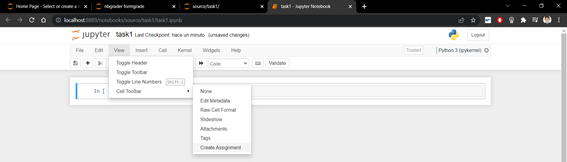
\includegraphics[width=1\textwidth]{img/prueba/prueba_6.png}
    \caption{Proceso de lanzamiento y creación 6}
\end{figure}

\item De esta manera las celdas tendrán diferentes formatos para la creación de la tarea:

\begin{figure}[H]
    \centering
    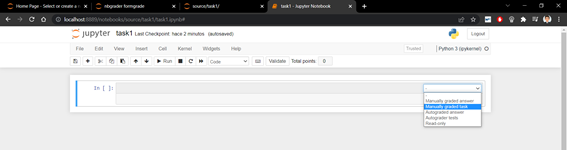
\includegraphics[width=1\textwidth]{img/prueba/prueba_7.png}
    \caption{Proceso de lanzamiento y creación 7}
\end{figure}

\item A continuación se puede crear nuestra primera prueba; se ha creado una prueba muy sencilla en la que se manda al alumno crear una función suma, para ello se crea una celda tipo “Autograded answer” en la que el profesor crea la función y deja entre los comentarios “\#\#\#BEGIN SOLUTION” y “\#\#\#END SOLUTION” la parte de código que el alumno ha de implementar. En la celda tipo “Autograded tests” se crean las pruebas para dicha función, estas pruebas están basadas es la ejecución de sentencias assert y se le ha de asignar una puntuación.

\begin{figure}[H]
    \centering
    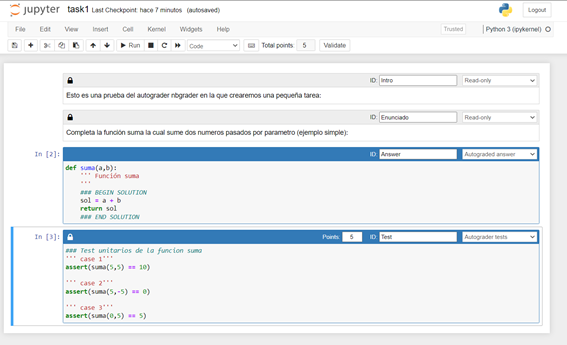
\includegraphics[width=1\textwidth]{img/prueba/prueba_8.png}
    \caption{Proceso de lanzamiento y creación 8}
\end{figure}

\item Una vez creadas las pruebas se ha de validar que el código del profesor es correcto y funciona por lo que se ha de hacer click en la casilla “validate” y en caso de que sea correcto recibiremos el siguiente mensaje:

\begin{figure}[H]
    \centering
    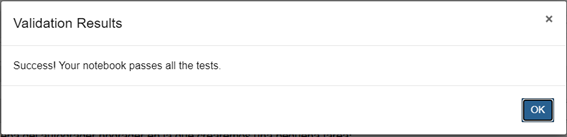
\includegraphics[width=1\textwidth]{img/prueba/prueba_9.png}
    \caption{Proceso de lanzamiento y creación 9}
\end{figure}

\item Una vez creado, volvemos a la sección de manejo de tareas:

\begin{figure}[H]
    \centering
    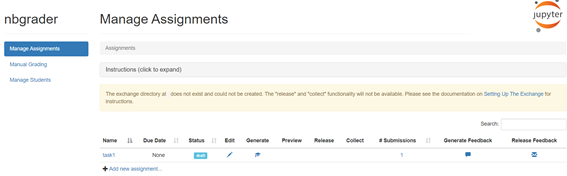
\includegraphics[width=1\textwidth]{img/prueba/prueba_10.png}
    \caption{Proceso de lanzamiento y creación 10}
\end{figure}

\item Para generar la tarea que sería entregada a los alumnos hacemos click en el icono de “generate” para la tarea correspondiente y recibiremos, en caso de funcionar correctamente, el siguiente mensaje:

\begin{figure}[H]
    \centering
    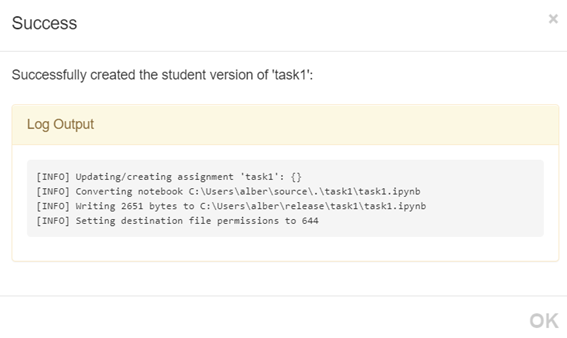
\includegraphics[width=1\textwidth]{img/prueba/prueba_11.png}
    \caption{Proceso de lanzamiento y creación 11}
\end{figure}

\item Una vez creado hacemos click en el apartado “preview” para previsualizarlo como un alumno lo vería:

\begin{figure}[H]
    \centering
    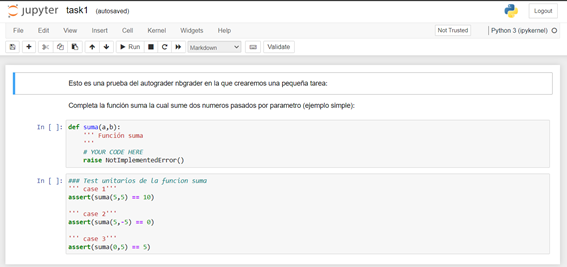
\includegraphics[width=1\textwidth]{img/prueba/prueba_12.png}
    \caption{Proceso de lanzamiento y creación 12}
\end{figure}

\item Como vemos en la casilla de la función suma, el contenido del código se ha modificado automáticamente para ser completado por el alumno.
Una vez hechos todos estos pasos ya tendríamos creada la tarea. En este momento nbgrader habrá generado automáticamente en el directorio raíz de tu equipo una nueva carpeta llamada “release” con la tarea correspondiente:

\begin{figure}[H]
    \centering
    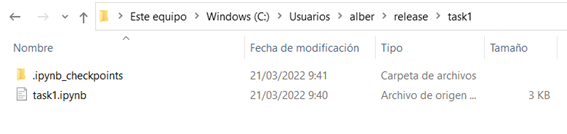
\includegraphics[width=1\textwidth]{img/prueba/prueba_13.png}
    \caption{Proceso de lanzamiento y creación 13}
\end{figure}

\item Este notebook será entregado al alumno para la realización de la tarea.

\end{enumerate}

\subsubsection{Realización de la tarea y corrección}

\begin{enumerate}
\item Una vez el alumno recibe la tarea y la completa: 

\begin{figure}[H]
    \centering
    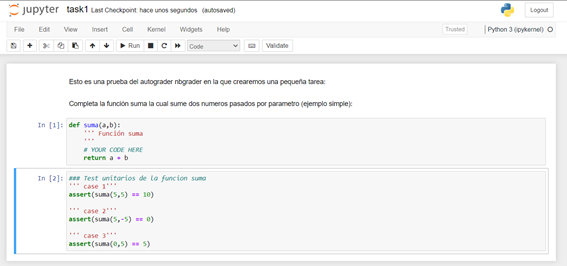
\includegraphics[width=1\textwidth]{img/prueba/prueba_14.png}
    \caption{Proceso de realización y corrección 1}
\end{figure}

\item Este puede comprobar su resultado haciendo click en el icono “validate” en caso de tener Nbgrader instalado:

\begin{figure}[H]
    \centering
    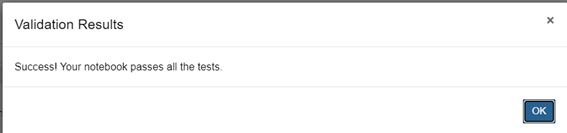
\includegraphics[width=0.8\textwidth]{img/prueba/prueba_15.png}
    \caption{Proceso de realización y corrección 2}
\end{figure}

\item Una vez haya acabado la tarea, la guardará y enviará de nuevo al profesor quien almacenará esta en el archivo dentro de submitted creado anteriormente para esa tarea:

\begin{figure}[H]
    \centering
    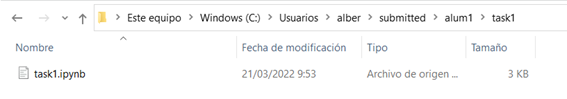
\includegraphics[width=1\textwidth]{img/prueba/prueba_16.png}
    \caption{Proceso de realización y corrección 3}
\end{figure}

\item Ahora el profesor accederá de nuevo al apartado de gestión de tareas:

\begin{figure}[H]
    \centering
    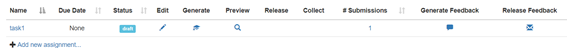
\includegraphics[width=1\textwidth]{img/prueba/prueba_17.png}
    \caption{Proceso de realización y corrección 4}
\end{figure}

\item Y accederá al apartado de submissions de la tarea:

\begin{figure}[H]
    \centering
    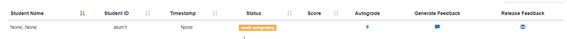
\includegraphics[width=1\textwidth]{img/prueba/prueba_18.png}
    \caption{Proceso de realización y corrección 5}
\end{figure}

\item Hacemos click en la opción “autograde”:

\begin{figure}[H]
    \centering
    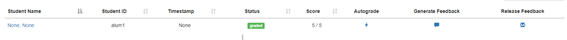
\includegraphics[width=1\textwidth]{img/prueba/prueba_19.png}
    \caption{Proceso de realización y corrección 6}
\end{figure}


\item Y como vemos se corrige automáticamente, en este caso el alumno ha aprobado. Adicionalmente si hacemos click en “generate feedback” nbgrader creará una carpeta “feedback” con documentos html con retroalimentación para el alumno:

\begin{figure}[H]
    \centering
    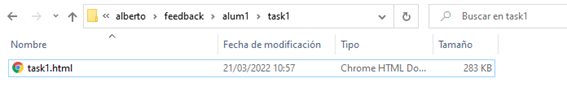
\includegraphics[width=1\textwidth]{img/prueba/prueba_20.png}
    \caption{Proceso de realización y corrección 7}
\end{figure}

\begin{figure}[H]
    \centering
    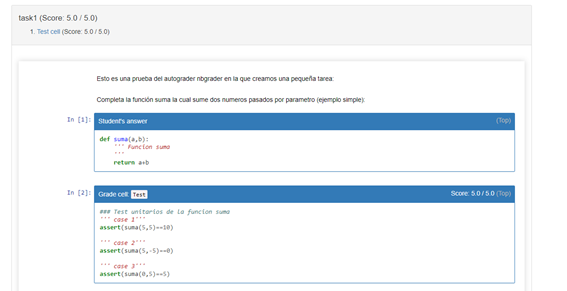
\includegraphics[width=1\textwidth]{img/prueba/prueba_21.png}
    \caption{Proceso de realización y corrección 8}
\end{figure}
\end{enumerate}

\subsection{Funcionamiento Nbgrader}
Como se ha visto en la prueba anterior, Nbgrader necesita una serie de directorios y archivos para su funcionamiento. La estructura de un curso sobre el que va a funcionar Nbgrader es la siguiente:
\begin{figure}[H]
    \centering
    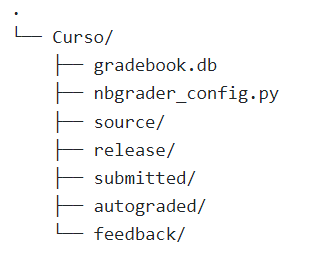
\includegraphics[scale=0.7]{img/imgs-memoria/NbgraderTree.PNG}
    \caption{Estructura Curso Nbgrader}
\end{figure}
\begin{itemize}
\item \textbf{gradebook.db:} Base de datos en la que Nbgrader almacena información sobre tareas, alumnos y entregas.
\item \textbf{nbgrader\_config.py:} Archivo de configuración de Nbgrader.
\item \textbf{source:} Directorio en el que se almacenan las tareas (notebooks) creadas por el profesor. Estos notebooks serán adaptados por Nbgrader para la generación de estos en versión alumno.
\item \textbf{release:} Directorio en el que se almacenan las tareas en versión del alumno tras ser generadas por Nbgrader.
\item \textbf{submitted:} Directorio en el que se almacenan las tareas entregadas por los alumnos.
\item \textbf{autograder:} Directorio en el que se almacenan las tareas corregidas.
\item \textbf{feedback:} Directorio en el que se almacenan los archivos feedback generados por Nbgrader de las tareas enviadas y corregidas.
\end{itemize}

En la siguiente tabla se muestran las diversas etapas en las que consiste el funcionamiento de Nbgrader con la información sobre los actores que realizan estas acciones, comandos utilizados, estructura de carpetas, archivos implicados y observaciones sobre estas:


\begin{landscape}
\begin{figure}[t]
    \hspace*{-2cm} 
    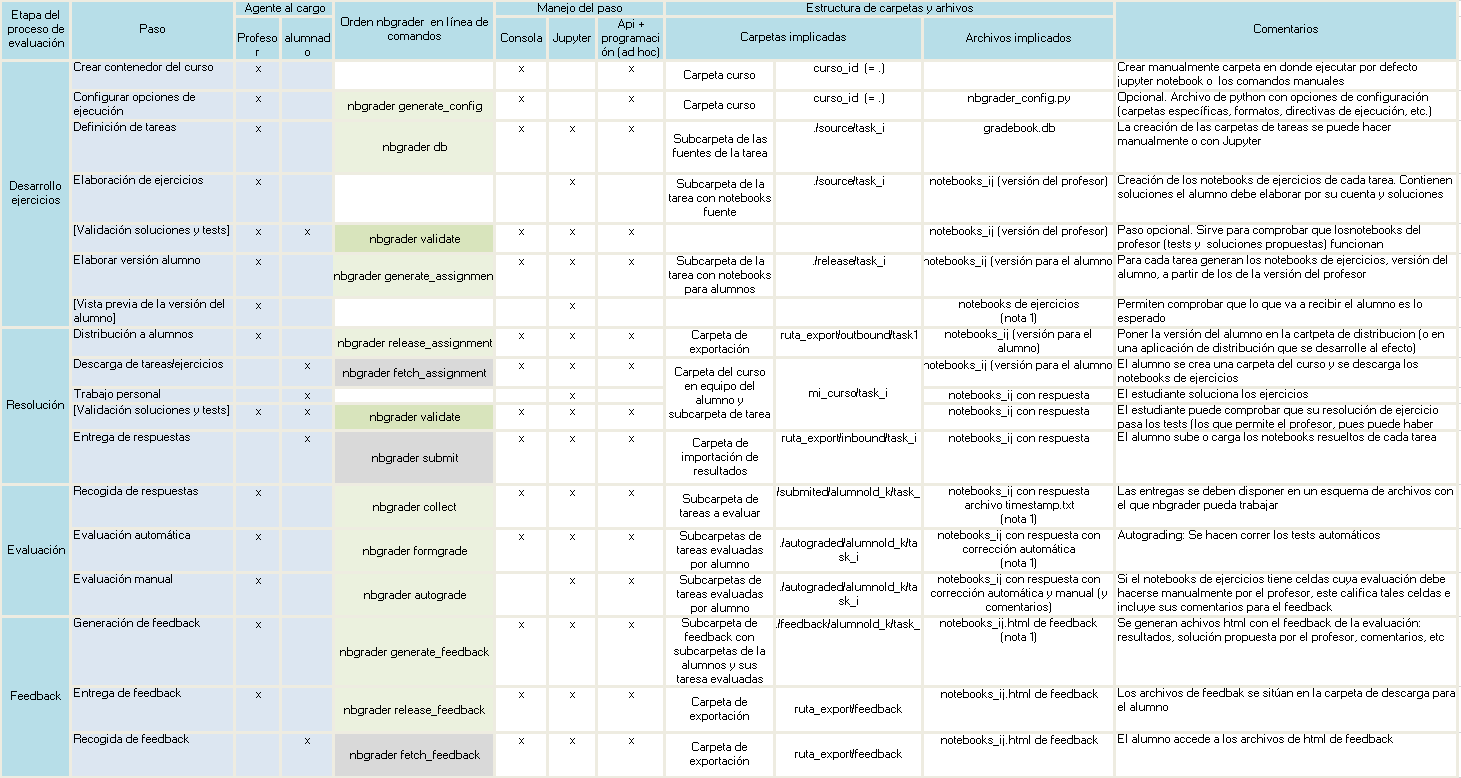
\includegraphics[scale=0.83]{img/imgs-memoria/Tabla_Nbgrader1.PNG}
    \caption{Tabla Nbgrader 1}
\end{figure}

\begin{figure}[t]
    \hspace*{-3cm} 
    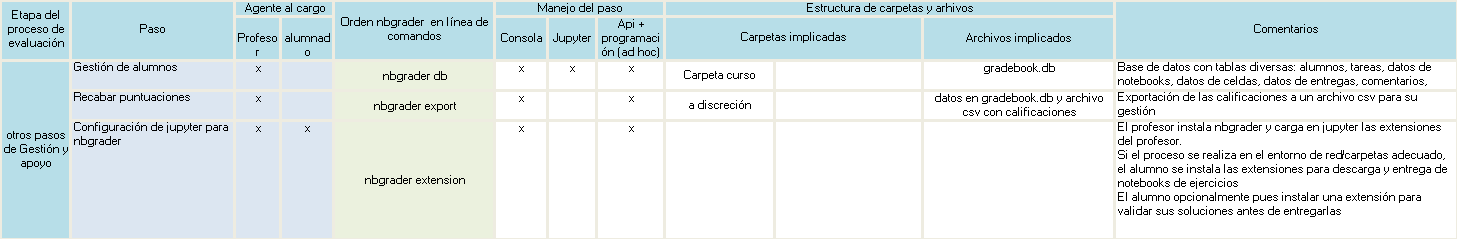
\includegraphics[scale=0.78]{img/imgs-memoria/Tabla_Nbgrader2.PNG}
    \caption{Tabla Nbgrader 2}
\end{figure}
\end{landscape}

\subsection{Creación de Cursos}
Ya se ha visto la estructura de archivos y directorios que necesita Nbgrader para su funcionamiento. Debido a esta dependencia estructural, la forma en la que ha sido implementada la creación de cursos dentro del proyecto ha consistido en el copiado y renombrado del directorio de un curso base el cual contiene todos los archivos y directorios necesarios para el funcionamiento de Nbgrader y la creación de tareas. Este curso se encuentra dentro de la carpeta \textit{courses} que es la propia carpeta en la que el resto de cursos serán añadidos:

\begin{figure}[H]
    \centering
    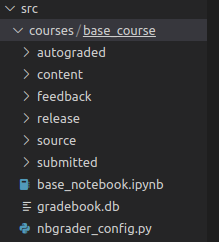
\includegraphics[scale=1]{img/imgs-memoria/base_course.PNG}
    \caption{Curso base}
\end{figure}

Adicionalmente, este curso base contiene el directorio \textit{content} cuya función es el almacenamiento de los archivos teóricos pertenecientes al curso.

El endpoint o método-ruta en el que es realizada esta acción es el denominado \textbf{teacher\_create\_course()} y concretamente la sección de código en la que se realiza esta acción es la siguiente:

\begin{figure}[H]
    \centering
    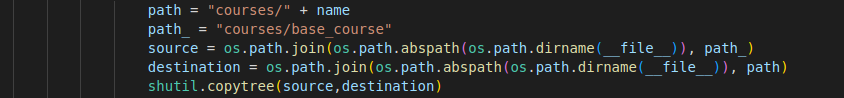
\includegraphics[scale=0.8]{img/imgs-memoria/Code_createCourse.PNG}
    \caption{Código creación curso}
\end{figure}


\subsection{Manejo de Nbgrader}
El manejo de Nbgrader dentro del proyecto se realiza mediante la clase \textbf{NbgraderManager} dentro del módulo \textbf{Management.py}.

\subsubsection{Construcción}
El constructor de esta clase es el siguiente:

\begin{figure}[H]
    \centering
    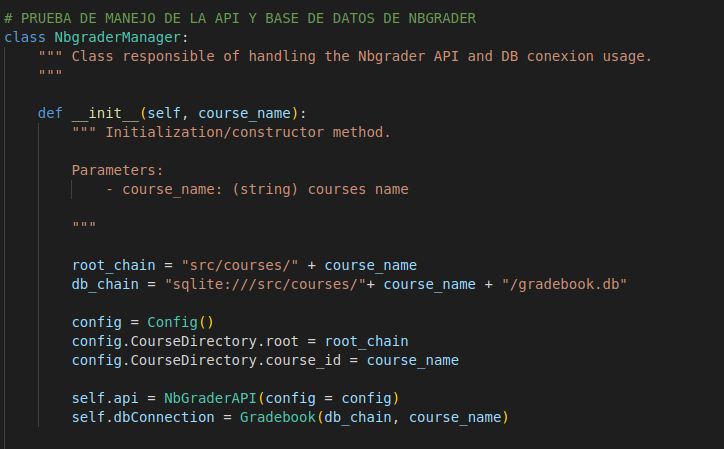
\includegraphics[scale=0.8]{img/imgs-memoria/ConstructorManager.PNG}
    \caption{Constructor manager}
\end{figure}

En este se está estableciendo la conexión con la base de datos \textit{gradebook.db} de Nbgrader dentro de la carpeta del curso pasado por parámetro sobre el que se van a realizar las acciones de Nbgrader. Adicionalmente se crea la variable de instancia de la API de Nbgrader por la que se ejecutarán las funciones de este. 

\subsubsection{Acciones más importantes}
Las operaciones más importantes del manager son las siguientes:

\begin{itemize}
\item \textbf{Grade:} Manda a la API de Nbgrader la realización de la corrección de una tarea accediendo a esta en la carpeta submitted del alumno pasado por parámetro y, en caso de tener éxito en la operación, accede a la base de datos para obtener la calificación obtenida, redondeándola sobre 10:
\begin{figure}[H]
    \centering
    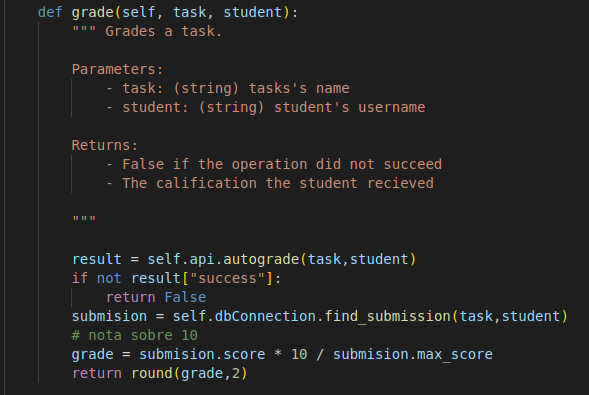
\includegraphics[scale=0.8]{img/imgs-memoria/Grade.PNG}
    \caption{Corrección de tarea}
\end{figure}

Este método es llamado desde el endpoint \textbf{student\_course()} al realizarse la entrega de una tarea por parte de un alumno.

\item \textbf{Create assigment:} Manda a la API de Nbgrader la generación de una tarea en versión de estudiantes. Para ello, accede a la tarea dentro de la carpeta source del curso:
\begin{figure}[H]
    \centering
    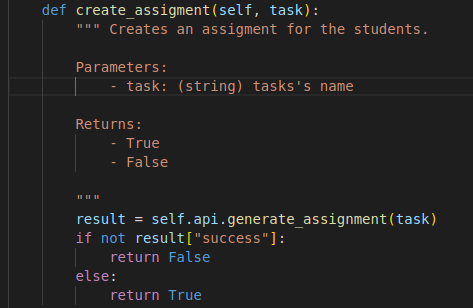
\includegraphics[scale=0.8]{img/imgs-memoria/CrearTarea.PNG}
    \caption{Generación de tarea para los alumnos}
\end{figure}

Este método es llamado cuando un profesor crea una sección de contenido de forma directa en la que entrega el notebook tarea creado previamente, acción realizada en el endpoint \textbf{teacher\_create\_section(course)}. O cuando el profesor ordena la publicación de una sección de contenido no publicada, acción realizada en el endpoint \textbf{publish\_section(course,section)}.

\item \textbf{Generate feedback:} Manda a la API de Nbgrader la generación del documento feedback de una tarea entregada por un alumno:

\begin{figure}[H]
    \centering
    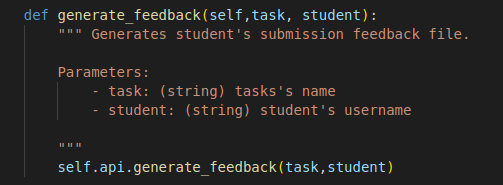
\includegraphics[scale=0.8]{img/imgs-memoria/generateFeedback.PNG}
    \caption{Generación de feedback}
\end{figure}

Este método es llamado tras la correcta corrección automática de una tarea al ser entregada por un alumno en el endpoint \textbf{student\_course()}.

\end{itemize}

\subsection{Creación de tareas desde la plataforma}

Ya ha sido mencionado con anterioridad el hecho de que una de las funcionalidades de la plataforma consistía en permitir a los profesores la creación de tareas desde la propia plataforma. Para lograr esto fueron añadidas las denominadas \textbf{Secciones no publicadas}. Estas secciones son creadas por el profesor dentro de uno de sus cursos y son solo visualizables por él y no por los alumnos, hasta su publicación o descarte. Al crearse una sección no publicada por un profesor, este define el nombre que tendrá el notebook tarea la cual es incluida en la carpeta \textit{source} del curso. Posteriormente, el profesor puede ver el listado de las secciones no publicadas del curso y acceder a la tarea que desee editar, momento en el que se le abrirá en su navegador una nueva pestaña en la que se está accediendo, mediante la ejecución remota de Jupyter Notebook, al notebook específico. Para lograr esto, Jupyter Notebook junto con Nbgrader se encuentra instalado dentro del propio proyecto y es ejecutado remótamente desde el momento inicial en el que la app es iniciada. Los comandos para lograr esto son los siguientes:

\begin{figure}[H]
    \centering
    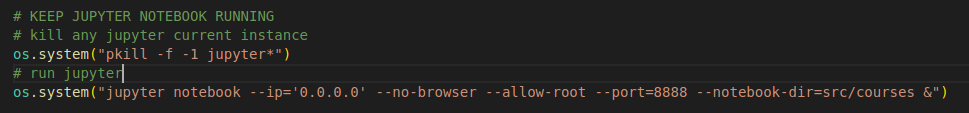
\includegraphics[scale=0.8]{img/imgs-memoria/RunJupyter.PNG}
    \caption{Ejecución de Jupyter}
\end{figure}

Para lograr la apertura del notebook tarea concreto que el profesor desea editar, se incluye la siguiente línea de código dentro del template de vistas de secciones sin publicar \textbf{unreleased\_sections.html}: 

\begin{figure}[H]
    \hspace*{-1.5cm} 
    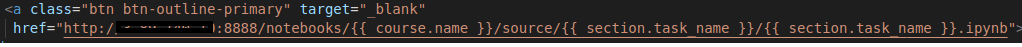
\includegraphics[scale=0.8]{img/imgs-memoria/AbrirNotebook.PNG}
    \caption{Apertura Notebook}
\end{figure}

Esta se encarga de abrir en una nueva pestaña el notebook específico, introduciendo la URL de este. Para ello se ha tenido que introducir la IP específica de la ruta de ejecución remota de nuestro Jupyter Notebook (la cual ha sido ocultada en esta imagen por seguridad), por ello, se debía conocer con anterioridad la IP sobre la que nuestra plataforma ha sido desplegada.

Cuando un profesor decide publicar una sección no publicada, la orden de generación de tarea es llamada, cogiendo el archivo correspondiente a esa sección en el fichero \textit{source} y generando dentro de \textit{release} la versión correspondiente a los alumnos. 


\subsubsection{Librerías y métodos relevantes utilizados}
En esta sección van a ser descritas algunas de las librerías y métodos más relevantes utilizados en el proyecto junto con su utilidad dentro del mismo:
\begin{itemize}
\item \textbf{os:} El módulo de Python os permite el uso de funcionalidades de sistema operativo de forma versatil. En nuestro proyecto, los métodos y módulos derivados de este utilizados han sido:
    \begin{itemize}
        \item \textbf{system:} Ejecución de comandos de sistema operativo. Ha sido utilizado para el lanzamiento de Jupyter Notebook desde el proyecto.
        \item \textbf{remove:} Método de borrado de ficheros dentro de un directorio. Ha sido utilizado para el borrado de envíos, borrado de archivos de contenido teórico y tareas dentro de los directorios \textit{source} de los cursos en la cancelación de secciones, borrado de archivos de contenido teórico en la eliminación de secciones y borrado de tareas en la entrega de las mismas por los alumnos en caso de no haberse podido realizar el autograding por problemas en ella.
        \item \textbf{path:} Modulo de manejo de rutas de archivos y directorios.
        \item \textbf{mkdir:} Método de creación de directorios. Ha sido utilizado para la creación de directorios fundamentales para el funcionamiento de Nbgrader.
        \item \textbf{rename:} Método de renombrado de archivos. Ha sido utilizado para el renombre de archivos en la creación de tareas de secciones no publicadas, tras realizarse la copia del notebook base encontrado en cada curso.
    \end{itemize}
\item \textbf{shutil:} El módulo de Python shutil permite realizar Operaciones de archivos de alto nivel. En nuestro proyecto, los métodos y módulos derivados de este utilizados han sido:
    \begin{itemize}
        \item \textbf{rmtree:} Método de borrado de rutas de directorios. Ha sido utilizado para el borrado de carpetas de alumnos dentro de los directorios \textit{feedback} y \textit{submitted} en el borrado de alumnos o extracción de los mismos de un curso, borrado de directorios que habían sido creados con anterioridad en la creación de secciones que han dado error de generación de tarea, cancelación de secciones no publicadas, borrado de cursos, eliminación de secciones y actividades similares.
        \item \textbf{copytree:} Método de copiado de árboles de archivos. Ha sido utilizado en la creación de nuevos cursos.
        \item \textbf{copy:} Método de copiado de archivos. Ha sido utilizado en la creación de nuevas tareas.
    \end{itemize}
\item \textbf{flask.send\_from\_directory():} Método de Flask para el envío de ficheros de un directorio. Utilizado para la descarga de archivos por parte de los usuarios.
\end{itemize}

\subsection{Montaje en Docker}

El Dockerfile a partir del que se ha generado la imagen del contenedor en el que ha sido instalada nuestra plataforma es el siguiente:


\begin{figure}[H]
    \centering
    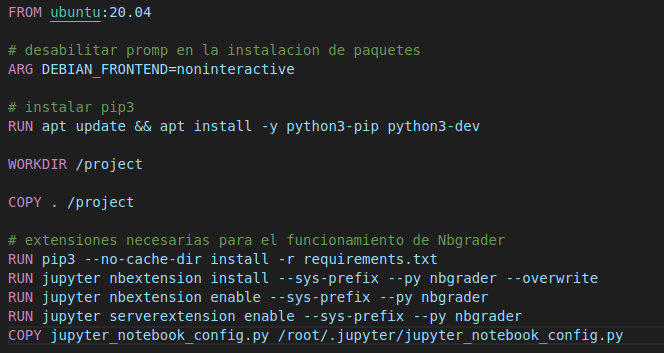
\includegraphics[scale=0.9]{img/imgs-memoria/Dockerfile.PNG}
    \caption{Dockerfile}
\end{figure}

En este se está ordenando la copia del proyecto junto con la instalación de todas sus dependencias software para su correcto funcionamiento. Adicionalmente, es introducida en la ruta de configuración de Jupyter Notebook el fichero \textbf{jupyter\_notebook\_config.py} el cual ha sido modificado deshabilitando la apertura de terminales y el botón de parada del kernel de ejecución para, en caso de que un profesor intente pararlo, este no pueda ya que esto generaría un problema en la edición de tareas desde la plataforma.

Una vez creada la imagen del contenedor a partir del dockerfile mediante la ejecución del comando \textbf{docker build -t "nombre\_imagen" .}.Este ha de ser ejecutado realizando el mapeo de puertos adecuado. Nuestra aplicación flask es lanzada a través del puerto local 5000 y Jupyter Notebook es ejecutado a través del 8888, por ello, el comando de construcción del contenedor con el mapeo de puertos correcto sería: \textbf{docker run -d -t --name=*nombre* -p *puerto de salida deseado para flask*:5000 -p *puerto de salida deseado para Jupyter*:8888 *nombre\_imagen*}. Una vez esté corriendo el contenedor con el mapeo de puertos correcto, se ha de acceder a este mediante el comando: \textbf{docker exec -ti *nombre* bash}.


Al ser ejecutado Jupyter de forma remota y accedido en un navegador web por primera vez, Jupyter pide al usuario que introduzca un token que este genera de forma automática, o una contraseña previamente establecida como forma de seguridad ante el intento de acceso a usuarios no autorizados. Puesto que los profesores que accedan de forma remota a Jupyter no tendrán acceso a este token generado automáticamente dentro del contenedor Docker, se ha de establecer una contraseña previa al lanzamiento de la aplicación. Para ello, una vez instalado el proyecto dentro del correspondiente contenedor Docker, se ha de establecer una contraseña mediante el comando \textbf{jupyter notebook password}. En el caso de nuestra plataforma, la contraseña que los profesores tendrán que introducir la primera vez que accedan a jupyter al crear o editar una tarea de forma remota será la palabra "teacher".

Una vez realizado el paso previo nuestra aplicación estaría lista para su ejecución desde el contenedor, acción que es realizada mediante la ejecución del comando \textbf{python3 app.py}. Tras esto nuestra aplicación podrá ser accesible de forma local en un navegador en la dirección \textbf{http://localhost:5000}.


\subsection{Riesgo de la ejecución remota de Jupyter Notebook}
El hecho de estar ejecutando jupyter notebook de forma remota con el fin de hacer posible la edición de tareas supone un inconveniente de seguridad. Este inconveniente consiste en que en el momento en el que un profesor está editando una tarea, este puede retroceder en el árbol de archivos de jupyter notebook, viendo así carpetas correspondientes al funcionamiento interno de los cursos:

\begin{figure}[H]
    \centering
    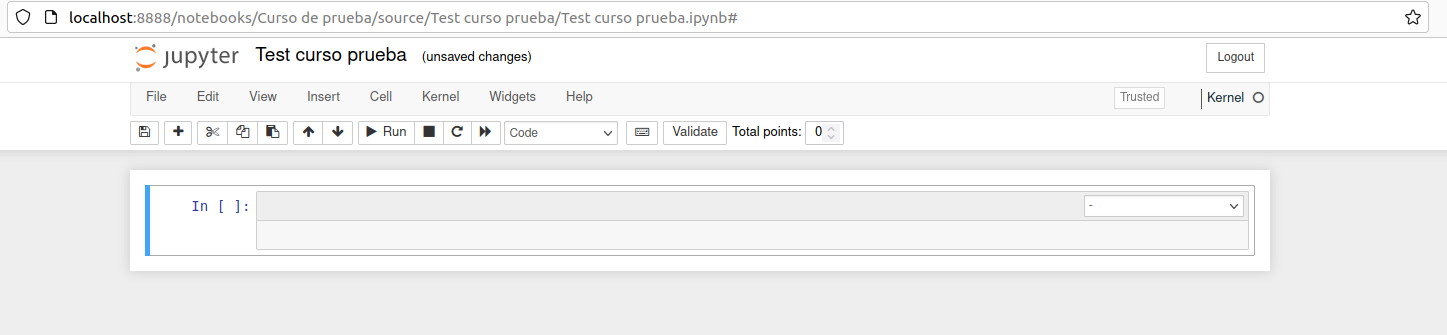
\includegraphics[width=14cm]{img/imgs-memoria/EdicionTarea.PNG}
    \caption{Edición de tarea}
\end{figure}

\begin{figure}[H]
    \centering
    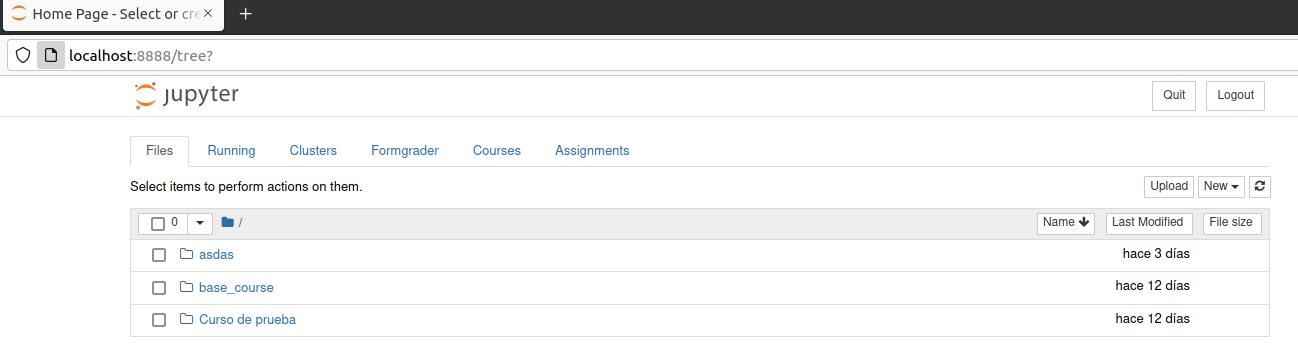
\includegraphics[width=14cm]{img/imgs-memoria/arbol archivos.PNG}
    \caption{Acceso carpetas de cursos}
\end{figure}

Como se puede ver en las imágenes anteriores, el profesor ha pasado de editar una tarea a ver las carpetas de los cursos de la página retrocediendo en la ruta de archivos de Jupyter. Este incoveniente de seguridad no es especialmente preocupante al ser los propios profesores quienes pueden acceder a estos archivos, pero es la principal razón por la que no se permite a los alumnos contestar a las tareas desde la propia web, sino que han de resoverlas de forma local habiéndose descargado la tarea. Si un alumno pudiera realizar esta acción, tendría acceso a todos los contenidos de los cursos incluidas las versiones de las tareas del profesor, lo que podría dar lugar a la realización de trampas para superar las tareas o incluso problemas de funcionamiento de la plataforma en el caso de que estos decidieran eliminar algún directorio o archivo. La resolución de este problema ha sido propuesta como una posible futura línea de trabajo en el apartado de conclusiones y futuras líneas de trabajo de la memoria.

\section{Instalación, ejecución y despliegue del proyecto}

\subsection{Instalación}
Puesto que se ha hecho uso de la herramienta VirtualEnv la instalación de nuestro proyecto \textbf{en un ambiente de desarrollo Ubuntu / Linux} es una tarea muy sencilla. Para ello simplemente se ha de clonar el repositorio del mismo el cual tiene incluida la carpeta env correspondiente a esta herramienta.

\subsection{Ejecución desde el entorno de desarrollo}

Para la ejecución de nuestra aplicación de forma local en el ambiente de desarrollo se ha de activar el ambiente virtual mediante el comando \textbf{source env/bin/activate} desde el directorio raíz del proyecto. Una vez hecho esto, nuestra aplicación puede ser lanzada mediante el comando \textbf{python3 app.py}.

Adicionalmente, puesto que el estado final en el que se encuentra el proyecto dentro del repositorio está pensado para el despliegue directo de la plataforma, se puede activar dentro del archivo de lanzamiento \textbf{app.py} el modo de depuración, asignando el valor ''True'' al parámetro ''Debug'' del método de ejecución Flask de la aplicación:

\begin{figure}[H]
    \centering
    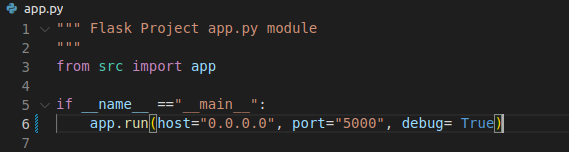
\includegraphics[scale=0.9]{img/imgs-memoria/DebugOn.PNG}
    \caption{Modo de depuración}
\end{figure}

\subsection{Despliegue}
La plataforma ha sido desplegada en una instancia EC2 de Amazon Web Service. En este apartado se va a explicar el proceso seguido para lograrlo en caso de que futuros programadores quieren realizar el mismo tipo de despliegue:

\begin{itemize}
\item Creación de la instancia t2.micro con imagen Amazon Linux gratuita de arquitectura 64 bits, par de claves RSA y formato de archivo pem y permitiendo el trafico HTTP desde internet.

\item Acceso a la instancia como cliente SSH. 

Comando: \textbf{ssh -i *Tu\_Archivo\_Clave.pem* ec2-user@ec2-3-89-140-10.compute-1.amazonaws.com}

\item Instalación de Docker y Git dentro de la instancia. Comandos: \textbf{sudo amazon-linux-extras install docker} y \textbf{sudo yum install Git}

\item Clonación del repositorio. Comando \textbf{Git clone *url*}

\item Asignación de permiso al usuario ec-2. Comando \textbf{sudo usermod -a -G docker ec2-user}.

\item Salida y vuelta a entrar a la instancia para la correcta asignación de permisos.

\item Creación de la imagen mediante docker build.

\item Lanzamiento del contenedor dentro de la instancia con el mapeo correcto de puertos. El puerto de salida de la plataforma Flask sobre el que se accederá a esta queda a elección del programador, en nuestro caso ha sido seleccionado el puerto 80. El puerto de salida de Jupyter Notebook ha de ser el 8888 por obligación ya que es hacia el que la plataforma redirecciona al abrir las tareas. 

\item Acceso al contenedor, establecimiento de la contraseña de Jupyter Notebook y lanzamiento de la aplicación como ha sido descrito en el apartado de Montaje en Docker del Manual del programador.

\item Adición de las dos reglas de entrada correspondientes a los dos puertos de nuestra plataforma dentro del grupo de seguridad de la instancia EC2. Tipo de reglas TCP personalizado y puertos 8888 (Jupyter Notebook) y el asignado a la salida de la aplicación Flask.

\item Salida de la instancia.
\end{itemize}

Una vez realizados los siguientes pasos nuestra plataforma será accesible en la url: \textbf{http://*IP\_INSTANCIA*:80}.